\documentclass[12pt]{article}

\usepackage{amsmath}
\usepackage{xcolor}
\usepackage{graphicx}

\newcommand{\alert}[1]{{\color{red}#1}}
\newcommand{\svdone}{{\tt dgesdd}$_1$\xspace}
\newcommand{\svdtwo}{{\tt dgesdd$_2$}\xspace}
\newcommand{\svdthree}{{\tt dgesdd$_3$}\xspace}
\newcommand{\svdfour}{{\tt dgesdd$_4$}\xspace}
\newcommand{\svdfive}{{\tt dgesdd$_5$}\xspace}
\newcommand{\svdsix}{{\tt dgesdd$_6$}\xspace}


\title{Response to the Reviewers}
\author{Joshua Garland, Ryan James, and Elizabeth Bradley}
\date{\today}

\begin{document}

\maketitle

\section*{Response to the First Referee}

\emph{In this manuscript the authors present a way to explore the
  relationship between predictability and complexity across a broad
  (but not complete) array of forecast strategies such as random walk
  (last value), na\"ive (average value), regression based (ARIMA) and
  a nonlinear method based on state space reconstruction (LMA). They
  use weighted permutation entropy as a criterion/index of predictive
  structure in the time series and illustrate their approach on eight
  real-world datasets derived from three different systems (computer
  performance traces).}

\emph{Overall the manuscript is well written and clearly
  understandable. The analysis seems to be carried out carefully and
  the conclusions drawn are quite reasonable. While I don't get the
  impression that this is a breakthrough paper I can still recommend
  the manuscript for publication in PRE if the issues listed below are
  addressed thoroughly.}

We thank the reviewer for their kind words and appreciate the time
they put into reviewing our work.

\noindent\emph{Major issues:}

\emph{I don't get the reason for normalizing the three methods by the
  random walk method (for example in Table I). As the authors write
  themselves this makes the indicator vulnerable to a bias caused by
  the high influence of this (arbitrarily selected) reference
  method. Why not just use a non-referential estimator, which then
  would also allow to compare the inherent predictability of different
  systems (as it is now the values obtained for each systems are
  strongly influenced by the random walk estimate on that particular
  system and thus can not be compared). This will also change the
  results of the fitting (the authors explicitly exclude one value
  because of the effect caused by the normalization). And it is not
  that the random walk predictor is the one standard method that all
  other methods have to compete against.}

No error metric is perfect.  For our purposes, we needed one that was
scale free and comparable across different time series.  While MASE
has its drawbacks, it was a very good fit to those requirements.  In
our opinion, this outweighed its disadvantages.  There is a great deal
of discussion of this cluster of issues in [Hyndman and Koehler, 2006]
\alert{[[(our reference [21])]]}.  If the reviewer thinks that it
would strengthen our paper, we can recapitulate some of that material
in our Section IVD.

Note that the fit in the revised version does not omit any points.

\smallskip

\emph{In many parts the article reads almost like a review. There is a
  lot of unnecessary redundancy (the entropy rate is quite low). In
  particular, the main point (``The aim of the paper is not ... but
  ...'') is repeated far too many times. The paper while easy to read
  could be shortened considerably without any loss of information.}

Due to the broad selection of fields that this work draws upon, we
thought it necessary to provide background for readers who might not
be familiar with all of them.  While this necessitated some
redundancy, we have made an effort to trim the fat and make the review
portions more streamlined.

\noindent\emph{Minor issues:}

\emph{Page 1: Why mention the `halting problem'? I don't see a
  straightforward connection to the problem at hand. The only
  connection is `undecidability' but there are many other examples for
  that.}

This is an important issue to the computer-science community, but we
have taken the reviewer's advice that it is less so for Physical
Review E---and hence removed it.

% Our intent in mentioning this theoretical result was to side-step the
% possible response of simply ``always use the most sophisticated
% prediction scheme''. This corollary implies that no matter how
% sophisticated and broad a scheme we construct, it will not be the
% optimal one for some time series. Thus there is a real need for
% determining when a better scheme exists. \alert{We have modified the
%   paragraph to make this point more clear.}

\smallskip

\emph{Page 10: `error between the predictions and the true continuations'
$\rightarrow$ `error of the predictions with respect to the true continuations'
Figure 6 on Page 11: It would be more intuitive to turn this into a `table of
figures' with the four methods as row labels on the left and the three systems
as column labels at the top. Also: Caption `for forecast of ... and all four
prediction strategies'.}

We have modified the text as the reviewer suggested and agree that it
reads more clearly now. We have also modified the figure as suggested.

\smallskip

\emph{First equation on Page 14: Shouldn't the index $j$ run from $i+1$ to
$i+\ell$ (instead of from $i$ to $i+\ell$)? You normalize by $\ell$ (not
$\ell+1$) values.}

Thank you for catching our mistake; we have corrected the equation.

\smallskip

\emph{Page 19: ``There are some exceptions: [...] Conversely, forecast errors
for the \texttt{col\_major} and \texttt{dgesdd$_5$} signals are higher than the
corresponding WPEs suggest --- except for the nonlinear LMA predictor.'' This is
not really an exception. As mentioned by the authors before, in general, the
result only holds under the assumption that a reasonably good model has been
used for the prediction. But for ill-matched datasets and models like in the
cases mentioned above this is just not the case so it is not a surprise that the
forecast errors are higher.}

You are absolutely correct and we've adjusted the text accordingly.

\section*{Response to the Second Referee}

We thank the reviewer for taking the time to read our paper and
provide us with valuable feedback.  The questions raised in this
review caused us to completely rethink the results, the fits, the
findings, and the conclusions---hence the long delay in resubmitting
this new version, the amount of rewritten material in the manuscript,
and the length of this response letter.

\smallskip

\emph{The problem of time series prediction is considered in the paper
  of J.  Garland et al. Namely, the authors suggest to quantify
  predictability in advance (before using any concrete prediction
  scheme) based on the complexity estimate (weighted permutation
  entropy, WPE). They hypothesize that WPE is related to the best
  possible prediction error in a simple way. For several benchmark
  time series (reflecting variations of a computer performance during
  execution of different tasks), they obtain estimates of WPE and
  prediction error (the least one over four techniques), and build a
  linear regression using seven or eight resulting data points. They
  suppose that the obtained linear function can be used to ``predict''
  the best prediction error from the model-free WPE estimate.  Thus,
  the authors finally assume (as could be seen from the last section)
  that WPE and optimal prediction error for all systems are related
  via the same universal linear function with fixed coefficients. This
  is what I can understand from the entire paper, though the problem
  is not so definitely described in the Introduction.}

We have modified the introduction in order to define our goals more
clearly.

\smallskip

\emph{I think that the possibility to estimate the best prediction
  error in advance from a relatively simple WPE characteristic would
  be interesting and useful, if it could hold true for a wide class of
  systems. Such a question would deserve a careful study as that
  started in the presented work. However, I have a number of critical
  remarks and strongly doubt that the conjecture of the authors can be
  valid for a reasonably wide class of systems (not even speaking of
  ``all systems''). Other aspects of the paper are not so important,
  in my view, despite some of them are fresh and interesting
  (e.g. taking a computer as an object of prediction). My critical
  remarks are listed below.}

Computer dynamics spans the full range of behavior reported in the
nonlinear dynamics literature.  Standard nonlinear time-series
analysis of data from these systems has confirmed the existence of
fixed points, periodic orbits of different periods, chaotic
trajectories with various Lyapunov exponents, etc.  in their dynamics.
While it is certainly possible that the nonlinear dynamics of computer
performance is subtly different from the nonlinear dynamics of other
systems---in a manner that cannot be detected by traditional nonlinear
time-series analysis---we believe that our results will hold for time
series drawn from other physical systems.

We are certainly aware that this claim may not be true, however, and
we are in the process of the follow-up study suggested by the
reviewer.  We have found that the relationship posited in our paper
holds for a time series of voltages from a chaotic laser used in the
SFI prediction competition, for instance.  It also holds for various
paradigmatic systems, such as the H\'{e}non map, the Lorenz system,
and a white-noise process.  The image below is an augmented version of
our revised Figure 7 that includes all of these examples; details
about each series and about the effects upon the fit are described
later in this letter.

\begin{center}
    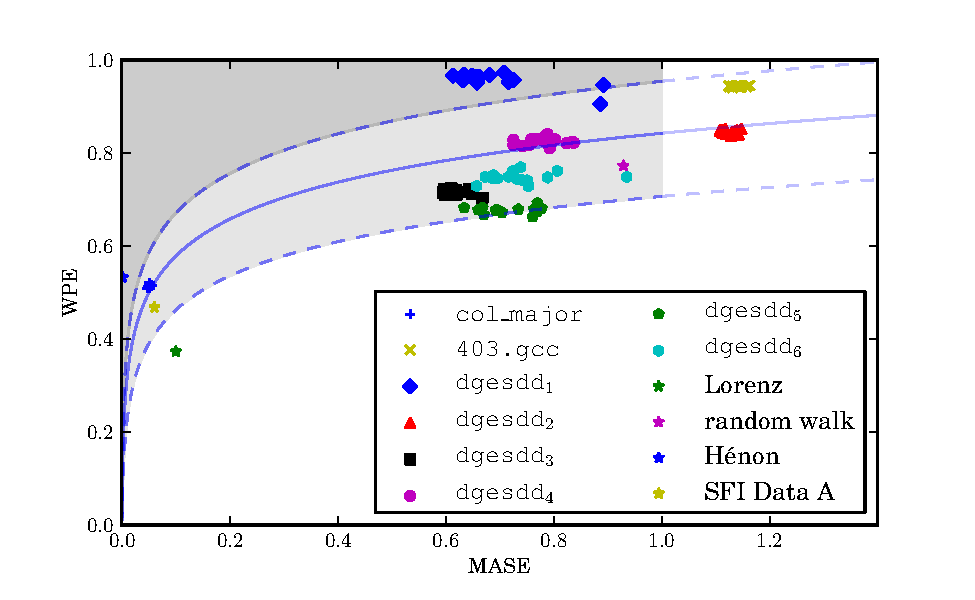
\includegraphics[width=0.8\columnwidth]{figs/new_prediction_vs_entropy_extras}
\end{center}

\noindent The dashed curve in this plot (and in Figure 6) was fit
\emph{solely on the computer performance data}.  Nonetheless, the
points from the other time series fall within a narrow band around the
fit.

Note that this fit ($y = a \log(b x + 1)$) is different than in the
submitted version.  A careful examination of the data and some careful
thought about the meaning and theoretical bounds of MASE---prompted by
the reviewer's questions---suggested that this was a better match to
the data.  This analysis and consideration is chronicled in the third
paragraph of the results section.  Finally, note that there are a lot
more points on this plot than in our original version; this is
discussed further below.

\smallskip

\emph{1) Introduction is too long, but the main problem is not
  formulated definitely enough. I see that the main point is the
  approximately linear (or at least one-to-one) relationship between
  WPE and the best prediction error. This aim is not claimed
  explicitly in the Introduction. All other aspects of the manuscript
  do not seem important enough to be published in a separate article.}

We have shortened the introduction and modified the manuscript
throughout to make it more clear that our goal was to derive a
practical criterion for best-case prediction error in a model-free
way, and to test it in the context of empirical data.  We have also
changed the title and abstract to line up with this goal.

\smallskip

\emph{2) In particular, two primary findings mentioned on page 2
  (Introduction) are formulated quite vaguely. The first part of the
  first finding reads ``(i) complexity of a noisy real-value time
  series is quantifiable by permutation entropy''. However, it seems
  obvious from the previous research, including that cited by the
  authors. The authors do not suggest PE or WPE here, they exploit
  them as previously known approaches. It was previously known that PE
  is an estimate of KS entropy as the authors also state. It was well
  known that KS entropy relates to predictability and, in this sense,
  it is a measure of complexity (see e.g. the work [G. Boffetta,
    M. Cencini, M. Falcioni, and A.  Vulpiani, ``Predictability: a way
    to characterize complexity'' // Physics Reports 356 (2002)
    367–474] which is not cited by the authors). Thus, the first part
  of the first finding does not provide any new information. The
  second part of the first finding reads ``(ii) complexity of the
  noisy real-valued time series is correlated with prediction accuracy
  of an appropriate predictor''.  However, it seems also obvious and
  directly follows from the definition of KS- entropy and its
  discussion in many papers including [Boffetta et al.] cited above.}

These claims have indeed been explored extensively in theory and in
toy models.  Our specific goal, which was not well explained in the
submitted version, was to show that those claims also hold---and can
be practically applied---in real-world time-series data that may
contain dynamical and/or observational noise.  This has not, to our
knowledge, received much attention in the literature.  We have added a
paragraph to the introduction that hopefully makes all of this more
clear.

We appreciate being informed about the Boffetta et al.  paper, and we
have included a discussion of it at the end of Section II.

\smallskip

\emph{3) By the way, the authors call ``fully complex'' the white
  noise process, i.e. they equate predictability and
  complexity. However, they do not even mention another approach to
  the notion of complexity which ascribes low complexity to the white
  noise [the works e.g. by C.R. Shalizi and J. Crutchfield carried out
    in the Santa Fe Institute from where one of the authors is]. It
  would be appropriate to mention that ambiguity of the notion of
  complexity if the latter plays an important role in many
  formulations of the authors.}

We have added a short discussion about the differences in notions and
definitions of complexity to Sections I and II and clarified the
working definition that we use in our work.

\smallskip

\emph{4) The second finding reads ``The way information is generated
  and processed internally by a system plays a crucial role in the
  success of different forecasting schema - and in the choice of which
  one is appropriate for a given time series''. This statement also
  looks trivial. Indeed, an optimal predictor for a linear stochastic
  system and low-dimensional nonlinear deterministic system are quite
  different (an AR model versus a local or global nonlinear model) due
  to different properties of the original systems. Thus, there is
  nothing to be proven here. Probably, the authors imply their
  particular benchmark signals (reflecting a computer behavior) but
  they do not claim that.  Thus, both primary findings seem to provide
  nothing new.}

The reviewer is absolutely right.  This finding, as it was originally
stated, is indeed trivial.  Our intent, as we have modified the text
to reflect, is that the appropriateness of a predictor for a given
time series can be discovered \emph{empirically}, via comparison of
its MASE value with the WPE value of the data.  Previous explorations
of predictability have used clean data and/or systems where the
generating process is known.  Our work makes neither of these
assumptions.

Given a linear stochastic system, a linear stochastic prediction model
should certainly be more productive than a nonlinear deterministic
prediction model.  But in real-world data, the generating process is
almost never known, and it can be very hard to evaluate a model that
one has constructed.  Standard methods like the AIC approach used in
ARIMA modeling make a choice from among a large class of possible
models.  These selection algorithms rarely have a ``none of these are
appropriate'' output; they simply choose the model that best satisfies
their built-in criteria---even if none of the models in the class are
really appropriate.

The challenge that this poses for a practitioner is to know whether
there is a mismatch between a particular time series from an unknown
system and a particular forecast model: i.e., whether one can do
better and should try another model, or whether the time series is so
complicated that the model under consideration is doing as well as one
could expect.  The curves and shaded regions on the WPE vs. MASE plots
in our paper are an empirical heuristic that should help practitioners
do that.

We appreciate the reviewer alerting us to our muddy wording and
thinking about these issues.  We have reworked the findings to clarify
matters and also added an explanatory paragraph directly following
those findings.

\smallskip

\emph{5) The benchmark system - a computer as an object of prediction
  - seems to be an unexpected and, probably, interesting choice but
  just as an additional illustration of a statement which should be
  first shown for well-controlled and well-understood paradigmatic
  systems (like low-dimensional maps or ordinary differential
  equations). Indeed, it is not known in advance what error one should
  expect for such a complicated object using a certain predictive
  technique, what technique is optimal or close to optimal, etc. If
  the main point of the research is the relationship between WPE and
  the best prediction error (if any), selection of such a complicated
  object as computer performance variations only introduces its own
  difficulties into the problem.}

Computers are indeed complicated objects, but we have studied their
dynamics extensively and established quite firmly that they are
garden-variety dynamical systems with surprisingly low-dimensional
dynamics [Mytkowicz et al. CHAOS, 2009].  Standard nonlinear
time-series analysis techniques on performance data measured from
running computers produce clean and consistent results, as mentioned
above: fixed points, bifurcations, chaotic attractors, and so on.

Well-known systems are certainly good test cases, but complicated,
unknown systems are where prediction really matters---especially
systems where a good prediction can make a practical difference (e.g.,
reallocation of resources in a computer to suit the dynamically
changing needs of a program).  The relationship posited in our paper,
as mentioned above, does indeed hold for paradigmatic systems like the
H\'{e}non map and the Lorenz equations.  We had not included these
examples in our paper because they simply confirmed well-known
results, and because our focus was on confirming those results in the
context of noisy, real-world data.  The penultimate paragraph of the
results section now explains that the WPE vs. MASE relationship for
these two synthetic examples (as well as for the Santa Fe ``A'' data
set, for a white-noise process, and for various nonlinear
transformations of our original data) all follow the empirically
determined pattern in our paper.

\smallskip

\emph{6) The description of the choice of the benchmark system in the
  Introduction is too long. On the other hand, if the computer signals
  are the main interest of the work, then it should be claimed
  explicitly. Then, the paper should be rewritten and submitted to a
  kind of engineering journals where it might well be of interest.}

The primary goal of this paper was to explore the relationship between
prediction error and WPE in noisy, real-world systems, and to assess
the practical applicability of this relationship.  Accordingly, we
have cut down on the level of detail regarding the benchmark system
and pointed interested readers to our other papers for the engineering
details.  We did not feel that removing all of this material would be
effective, however, because it helps the reader understand why this is
a good testbed for exploring the problem at hand.

\smallskip

\emph{7) As for the choice of the four prediction techniques, some of
  them seem superfluous. E.g. naive approach is just a global AR model
  of the zero order.  Random-walk is similar to the AR model of the
  first order where the coefficient is not estimated by the
  least-squares but set equal to 1 (or this is an ARIMA model with the
  first difference and ``zero ARMA part''). Inefficiencies of the
  ARIMA model as compared to those choices in the paper can represent
  an inappropriate procedure for the order selection rather than
  indicate inappropriateness of the entire ARIMA approach. Thus,
  linear ARIMA and nonlinear LMA might be sufficient (in combination
  with mathematical benchmark examples) to represent close-to-optimal
  prediction errors.}

It is certainly true that the naive and random-walk predictors can be
seen as subclasses of the ARIMA model family.  We have explicitly
included them, however, because they are used (sometimes to great
success) in practice, because that made for a more-comprehensive
exploration, and because of a subtle issue regarding model building
procedures.

The {\tt auto.arima} method that was used to build all of the ARIMA
models in this paper---another ``off the shelf'' method in the
modeling and prediction communities---follows the procedure outlined
in Section V B to choose values for the model parameters.  Sometimes
the choices made by that procedure (e.g., setting a particular
parameter to zero) produce a naive or random-walk predictor.  Our
method can help practioners know whether this is a good or bad thing.
If a particular model performs poorly, compared to what the WPE value
might suggest, it may be an indication that the chosen parameter
values were suboptimal---or even that no member of the ARIMA family
will work and one should try a different class of model.  A discussion
of these issues has been added to Section VI (page 18, left-hand
column, ``The discussion in the previous paragraph...'') in the hopes
of clarifying this completely valid concern and illustrating that this
is a feature of our proposed heuristic.

% Unfortunately the WPE value alone is insufficient to differentiate
% these two situations.  It can identify both, but cannot distinguish.

We have also changed the term used in the paper to {\tt auto.arima} in
order to make it clear that this refers not to the general class of
these models, but to a particular member of that class chosen via a
particular procedure.

\smallskip

\emph{8) Conditions for inefficiency of simple prediction schemes
  (like naive and random-walk) discussed in the paper look rather
  obvious as well and do not give new information. Is it the purpose
  of the paper to discuss when and where a concrete simple prediction
  scheme fails?}

This short paragraph in this paper, which explains the efficiencies
and inefficiencies of these schemes, was intended to serve two
purposes: first, to explain why we have included these simple
prediction schemes and not just the more-complicated ones; second, to
help in explaining the specific results described later in the paper.

\smallskip

\emph{9) A better justification of the prediction error metrics could
  be also in order if this work is continued. At least, comparison of
  prediction errors quantified with different metrics seems
  necessary. Especially, taking into account the following major
  concerns.}

We have extended the justification for our use of the MASE metric; see
the last paragraph in Section VI.  As mentioned there, the paper in
which MASE was introduced---\alert{[[our reference [21]]]}---includes
an extensive evaluation of this metric, as well as a comprehensive
comparison to other metrics.  If the reviewer thinks that it would
strengthen our paper, we can recapitulate more of that material in our
paper.  As part of our current work on this topic, we are evaluating
how other choices of metric affect the shape of our curves, but we
feel that a comprehensive study of this issue is best left as a sequel
to this work.

\smallskip

\noindent\emph{General remarks.}

\emph{I) Strict relationship between WPE and prediction error
  applicable to all systems is hardly possible. In particular, there
  is a notion of epsilon-entropy which tends to the KS entropy if
  epsilon (the cell size) tends to zero (see e.g.  [Boffetta et al.]
  cited above). For stochastic systems, the KS entropy is infinite and
  epsilon-entropy varies strongly with the scale epsilon. Seemingly,
  the permutation entropy estimate in this case will strongly depend
  on the choice of the word length L. The authors concentrate on L = 6
  and obtain coefficients of the regression between WPE and prediction
  error only for that choice and for their particular
  signals. However, other systems and other choices of L may easily
  lead to other regression coefficients so that deciding about the
  best possible prediction error from WPE seems impossible in
  general. It is good if such a decision is possible for a certain
  narrow class of systems. However, the authors do not even discuss to
  which class of systems their results apply.}

WPE values depend not only on wordlength, but also on \emph{data}
length, since one needs more data to get good statistics on the words
for the PE calculation if those words are longer.  These two
interacting knobs are not easy to set.  Perhaps as a result of this,
wordlength choices are rarely justified in the permutation entropy
literature.  The extent of the discussion in [Bandt \& Pompe, {\sl
    PRL}, 2002], for instance---the paper in which PE was
proposed---is ``Our entropies are calculated for different [$\ell$]
but we do not determine a limit for large [$\ell$], although this is
an interesting theoretical problem. For practical purposes, we
recommend 3\dots7...''  The corresponding discussion in [Cao {\sl et
    al.}, {\sl PRE}, 2004] reads ``In their paper, Bandt \& Pompe
recommended [$\ell$] of 3-7.  We often found that 3 and 4 may still be
too small, and a value of 5, 6, or 7 seems to be the most
suitable....''

The right thing to do, as we argued in the last paragraph of Section
V, is to compute PE across a \emph{range} of wordlengths ($\ell$) and
look for a flat spot in the curve of PE versus $\ell$.  We applied
that approach individually to each of the time series studied here to
choose a $\ell$ value that was appropriate to that particular trace.
(All of those values ended up being 6, which is consistent with the
informal arguments in previous papers, but that was not an \emph{a
  priori} or global choice.)  We conjecture that a systematic approach
like this will mitigate any variation in the results, thereby
preserving the shape of the WPE vs. MASE curve.  We have not yet
confirmed that conjecture, but we are working on it.

Regarding generality: the goal of this paper was to explore model-free
heuristics for empirical time-series data, where one does not know
anything about the underlying system.  In situations like this,
equivalence classes are difficult to define.  We addressed
this---insofar as is possible in an experimental context---by choosing
a range of time-series data sets whose behavior spans a wide range of
dynamical behaviors.  For all of these examples---as well as for the
49 additional ones
% \footnote{H\'{e}non, Lorenz, SFI A,
%  nonlinear transformations of the 45 svdone, svdtwo and signals}
constructed as a result of the reviewer's questions and described in
different parts of this response letter---the pattern in Figure 7
remained virtually unchanged.  This strongly suggests, but of course
does not prove, that our approach is general.  As the reviewer
suggested, this will require extensive study and evaluation in future
work.

\smallskip

\emph{II) PE is invariant under an invertible nonlinear change of
  variables. The prediction error measured as the authors suggest is
  not invariant. Thus, such a simple change of variables can lead, at
  least, to a change in regression coefficient between WPE and
  prediction error. Thus, the authors should also discuss to which
  variable for that class of systems their result apply. I think that
  the fact that the authors observe a certain regression line at all
  seems to be due to small number of different signals they consider
  (only 7 or 8 different data points, such a small number of points
  may lie approximately near a straight line by chance).}

Regarding the second part of this point: we have revised the fits in
Figures 6 and 7 in the paper, and the associated text, to include all
120 points.  As mentioned above, we have also moved from a linear fit
to a log fit of these points in order to better match the theoretical
relationship between MASE and WPE.  We now show and discuss the
one-$\sigma$ volume around that fit in an effort to emphasize that the
fundamental claim of the paper is not related to the crispness of the
fit.

Regarding the first part of this point: while PE is invariant under an
invertible nonlinear transformation of the values in the time series,
WPE is not---which amplifies the potential concerns about this issue.
To explore this, we performed the invertible nonlinear transformation
$f(x)=5e^{x(t)}$ on several of our traces ($x(t)=$ {\tt dgesdd}$_2$,
{\tt dgesdd}$_5$, and {\tt dgesdd}$_6$).  The image below shows WPE
vs. MASE results of the best predictor on these three traces, along
with those on the untransformed originals:

\begin{center}
    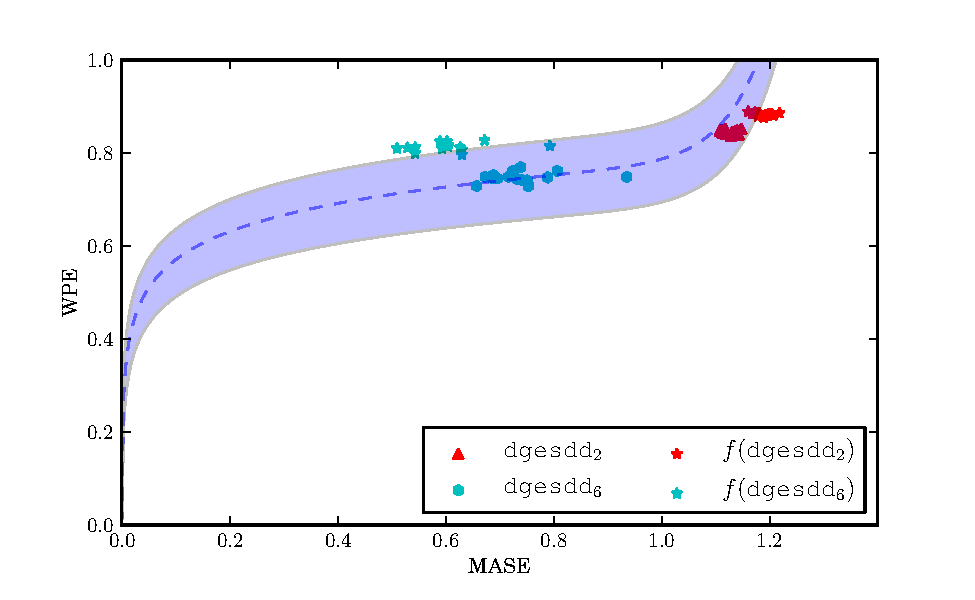
\includegraphics[width=0.8\columnwidth]{figs/nonlinear_transform_data}
\end{center}

The WPE vs. MASE points of the transformed data move---upwards,
generally---but they remain within the shaded region.  Indeed, the
values for the transformed version of {\tt dgesdd}$_5$ (dark-green
icons) move {\sl closer} to the curve.

This series of experiments supports our claims of generality: a
transformation like this effectively changes the generating process,
but does not affect the performance of our model-free heuristic.  And
the curves that capture that heuristic---which were derived from data
from a single computer-performance experiment---do not only hold for
traces from that experiment and transformed versions of them.  The
preliminary results of our broader study, currently underway, indicate
that they also hold for data from synthetic examples and for
real-world data from a different system.  The image below shows some
of these results:

\begin{center}
    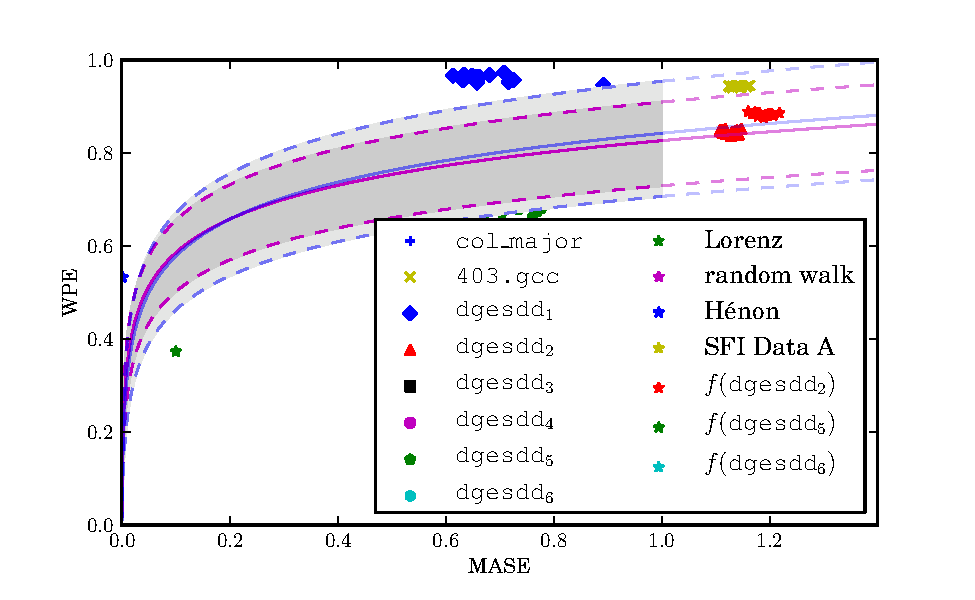
\includegraphics[width=0.8\columnwidth]{figs/new_prediction_vs_entropy_extras_with_nonlinear_all_points}
\end{center}

The blue fit lines here are derived from the original 120 traces; the
magenta one is fit to those traces plus the nonlinear transformations
of {\tt dgesdd}$_2$, {\tt dgesdd}$_5$, and {\tt dgesdd}$_6$, the $x$
coordinate of a 10,000-point orbit from the H\'{e}non map with $a=1.4$
and $b=0.3$, the $x$ coordinate of a 10,000-step 4th-order Runge-Kutta
solution of the Lorenz equations with $r=28, \; \sigma=10, \; b=8/3$
and $\Delta t=0.01$, a 10,000-step random-walk time series generated by
taking the cumulative sum of $\mu=0$, $\sigma=1$ Gaussian random
variables using Numpy ({\tt numpy.cumsum(numpy.random.normal(0.0, 1.0, size=10000))}),
and data set ``A'' from the Santa Fe Institute time-series competition
website.

Note that the inclusion of these additional 49 points hardly changed
the main central curve of the fit.  Indeed, doing so caused the
one-$\sigma$ volume of the fit to shrink (viz., the dashed magenta
curves inside the dashed blue curves).  \emph{That is, the additional
  points firmed up the findings.}  The magenta curve reflects a map, a
flow, a purely stochastic signal, a variety of real-world data from
two different systems (laser, computer), and nonlinear transformations
of the computer-performance data---again, supporting the generality of our
heuristic.

We are in the process of broadening this study to other systems,
transformations, and situations; in the meantime, we have added a
sentence about these preliminary results to the penultimate paragraph
in Section VI.

\smallskip

\emph{To summarize, the paper shows that the authors are well familiar
  with the entire topic and highly qualified, they overview some
  well-known facts (WPE, various prediction techniques, etc) and
  ``invent'' an unexpected test system (computer performance data),
  they report about their attempts to play around with all that
  staff. However, their results do not seem to provide any new
  information to a specialist. Probably, this work can be continued to
  get some more reliable results about concrete relationship between
  WPE and prediction error for certain classes of systems (however, I
  doubt that it is possible to derive any simple and widely applicable
  relationship like the linear function suggested by the
  authors). Seemingly, it should then be a new paper which can be
  hardly considered as a revised version of the present manuscript.}

It is our hope that these clarifications, the attendant modifications
to the paper, and the additional preliminary results that we included
in this rebuttal letter have convinced the reviewer that this
manuscript is appropriate for publication in PRE.

\end{document}
